% Options for packages loaded elsewhere
\PassOptionsToPackage{unicode}{hyperref}
\PassOptionsToPackage{hyphens}{url}
%
\documentclass[
  ignorenonframetext,
]{beamer}
\usepackage{pgfpages}
\setbeamertemplate{caption}[numbered]
\setbeamertemplate{caption label separator}{: }
\setbeamercolor{caption name}{fg=normal text.fg}
\beamertemplatenavigationsymbolsempty
% Prevent slide breaks in the middle of a paragraph
\widowpenalties 1 10000
\raggedbottom
\setbeamertemplate{part page}{
  \centering
  \begin{beamercolorbox}[sep=16pt,center]{part title}
    \usebeamerfont{part title}\insertpart\par
  \end{beamercolorbox}
}
\setbeamertemplate{section page}{
  \centering
  \begin{beamercolorbox}[sep=12pt,center]{part title}
    \usebeamerfont{section title}\insertsection\par
  \end{beamercolorbox}
}
\setbeamertemplate{subsection page}{
  \centering
  \begin{beamercolorbox}[sep=8pt,center]{part title}
    \usebeamerfont{subsection title}\insertsubsection\par
  \end{beamercolorbox}
}
\AtBeginPart{
  \frame{\partpage}
}
\AtBeginSection{
  \ifbibliography
  \else
    \frame{\sectionpage}
  \fi
}
\AtBeginSubsection{
  \frame{\subsectionpage}
}

\usepackage{amsmath,amssymb}
\usepackage{lmodern}
\usepackage{iftex}
\ifPDFTeX
  \usepackage[T1]{fontenc}
  \usepackage[utf8]{inputenc}
  \usepackage{textcomp} % provide euro and other symbols
\else % if luatex or xetex
  \usepackage{unicode-math}
  \defaultfontfeatures{Scale=MatchLowercase}
  \defaultfontfeatures[\rmfamily]{Ligatures=TeX,Scale=1}
\fi
% Use upquote if available, for straight quotes in verbatim environments
\IfFileExists{upquote.sty}{\usepackage{upquote}}{}
\IfFileExists{microtype.sty}{% use microtype if available
  \usepackage[]{microtype}
  \UseMicrotypeSet[protrusion]{basicmath} % disable protrusion for tt fonts
}{}
\makeatletter
\@ifundefined{KOMAClassName}{% if non-KOMA class
  \IfFileExists{parskip.sty}{%
    \usepackage{parskip}
  }{% else
    \setlength{\parindent}{0pt}
    \setlength{\parskip}{6pt plus 2pt minus 1pt}}
}{% if KOMA class
  \KOMAoptions{parskip=half}}
\makeatother
\usepackage{xcolor}
\newif\ifbibliography
\setlength{\emergencystretch}{3em} % prevent overfull lines
\setcounter{secnumdepth}{-\maxdimen} % remove section numbering


\providecommand{\tightlist}{%
  \setlength{\itemsep}{0pt}\setlength{\parskip}{0pt}}\usepackage{longtable,booktabs,array}
\usepackage{calc} % for calculating minipage widths
\usepackage{caption}
% Make caption package work with longtable
\makeatletter
\def\fnum@table{\tablename~\thetable}
\makeatother
\usepackage{graphicx}
\makeatletter
\def\maxwidth{\ifdim\Gin@nat@width>\linewidth\linewidth\else\Gin@nat@width\fi}
\def\maxheight{\ifdim\Gin@nat@height>\textheight\textheight\else\Gin@nat@height\fi}
\makeatother
% Scale images if necessary, so that they will not overflow the page
% margins by default, and it is still possible to overwrite the defaults
% using explicit options in \includegraphics[width, height, ...]{}
\setkeys{Gin}{width=\maxwidth,height=\maxheight,keepaspectratio}
% Set default figure placement to htbp
\makeatletter
\def\fps@figure{htbp}
\makeatother

\makeatletter
\makeatother
\makeatletter
\makeatother
\makeatletter
\@ifpackageloaded{caption}{}{\usepackage{caption}}
\AtBeginDocument{%
\ifdefined\contentsname
  \renewcommand*\contentsname{Table of contents}
\else
  \newcommand\contentsname{Table of contents}
\fi
\ifdefined\listfigurename
  \renewcommand*\listfigurename{List of Figures}
\else
  \newcommand\listfigurename{List of Figures}
\fi
\ifdefined\listtablename
  \renewcommand*\listtablename{List of Tables}
\else
  \newcommand\listtablename{List of Tables}
\fi
\ifdefined\figurename
  \renewcommand*\figurename{Figure}
\else
  \newcommand\figurename{Figure}
\fi
\ifdefined\tablename
  \renewcommand*\tablename{Table}
\else
  \newcommand\tablename{Table}
\fi
}
\@ifpackageloaded{float}{}{\usepackage{float}}
\floatstyle{ruled}
\@ifundefined{c@chapter}{\newfloat{codelisting}{h}{lop}}{\newfloat{codelisting}{h}{lop}[chapter]}
\floatname{codelisting}{Listing}
\newcommand*\listoflistings{\listof{codelisting}{List of Listings}}
\makeatother
\makeatletter
\@ifpackageloaded{caption}{}{\usepackage{caption}}
\@ifpackageloaded{subcaption}{}{\usepackage{subcaption}}
\makeatother
\makeatletter
\@ifpackageloaded{tcolorbox}{}{\usepackage[many]{tcolorbox}}
\makeatother
\makeatletter
\@ifundefined{shadecolor}{\definecolor{shadecolor}{rgb}{.97, .97, .97}}
\makeatother
\makeatletter
\makeatother
\ifLuaTeX
  \usepackage{selnolig}  % disable illegal ligatures
\fi
\IfFileExists{bookmark.sty}{\usepackage{bookmark}}{\usepackage{hyperref}}
\IfFileExists{xurl.sty}{\usepackage{xurl}}{} % add URL line breaks if available
\urlstyle{same} % disable monospaced font for URLs
\hypersetup{
  pdftitle={CSwR22 Group2 Bivariate Smoothing},
  pdfauthor={Isin Altinkaya, Dumitru Sebastian Pavel},
  hidelinks,
  pdfcreator={LaTeX via pandoc}}

\title{CSwR22 Group2 Bivariate Smoothing}
\author{Isin Altinkaya, Dumitru Sebastian Pavel}
\date{}

\begin{document}
\frame{\titlepage}
\ifdefined\Shaded\renewenvironment{Shaded}{\begin{tcolorbox}[frame hidden, breakable, boxrule=0pt, sharp corners, enhanced, borderline west={3pt}{0pt}{shadecolor}, interior hidden]}{\end{tcolorbox}}\fi

\hypertarget{introduction}{%
\section{Introduction}\label{introduction}}

\begin{frame}{Bivariate smoothing}
\protect\hypertarget{bivariate-smoothing}{}
\end{frame}

\begin{frame}[fragile]{Objectives}
\protect\hypertarget{objectives}{}
\begin{itemize}
\tightlist
\item
  Implement a smoothing spline smoother using LOOCV for selecting the
  tuning parameter \(\lambda\)
\item
  Test the accuracy of the implementation
\item
  Compare the results with \texttt{smooth.spline}
\item
  Code improvement
\item
  Benchmarking
\item
  Bottlenecks (profiling)
\item
  Test the implementation with real data and simulated data
\item
  Utilizing matrix decomposition in combination with LOOCV
\end{itemize}
\end{frame}

\begin{frame}{Theory (1/3)}
\protect\hypertarget{theory-13}{}
Leave one out cross validation. From the course, for a linear smoother:
\[LOOCV=\sum_i (y_i - \hat{f}^{-i}_i)^2=\sum_i (\frac{y_i - \hat{f}_i}{1 - S_{ii}})^2\]
\end{frame}

\begin{frame}{Theory (2/3)}
\protect\hypertarget{theory-23}{}
A linear smoother \(\hat{f}\) can be written as: \[\hat{f}=Sy\] Where
\(S\) is a matrix and \(y\) is the vector containing data (the labels).
\end{frame}

\begin{frame}{Theory (3/3)}
\protect\hypertarget{theory-33}{}
A spline smoother is written as:
\[\hat{f}=\Phi(\Phi^T\Phi + \lambda \Omega)^{-1}\Phi^Ty\] Where
\(S_{\lambda}=\Phi(\Phi^T\Phi + \lambda \Omega)^{-1}\Phi^T\).
\end{frame}

\begin{frame}[fragile]{Implementation: \(\Phi\)}
\protect\hypertarget{implementation-phi}{}
The matrix \(\Phi\) can be implemented as such:\\
\texttt{splineDesign(sort(c(rep(range(inner\_knots),\ 3),\ inner\_knots)),\ inner\_knots)}

Where \texttt{inner\_knots} are the knots given to the smoother.
\end{frame}

\begin{frame}{Implementation: \(\Omega\)}
\protect\hypertarget{implementation-omega}{}
The penalty matrix \(\Omega\) can be implemented as such:

Where the integrations are calculated using Simpson's rule.
\end{frame}

\begin{frame}{Implementation: \texttt{LOOCV}}
\protect\hypertarget{implementation-loocv}{}
\begin{enumerate}
\item
\end{enumerate}
\end{frame}

\begin{frame}{Implementation: Context}
\protect\hypertarget{implementation-context}{}
\end{frame}

\begin{frame}{Implementation: Context (visualization)}
\protect\hypertarget{implementation-context-visualization}{}
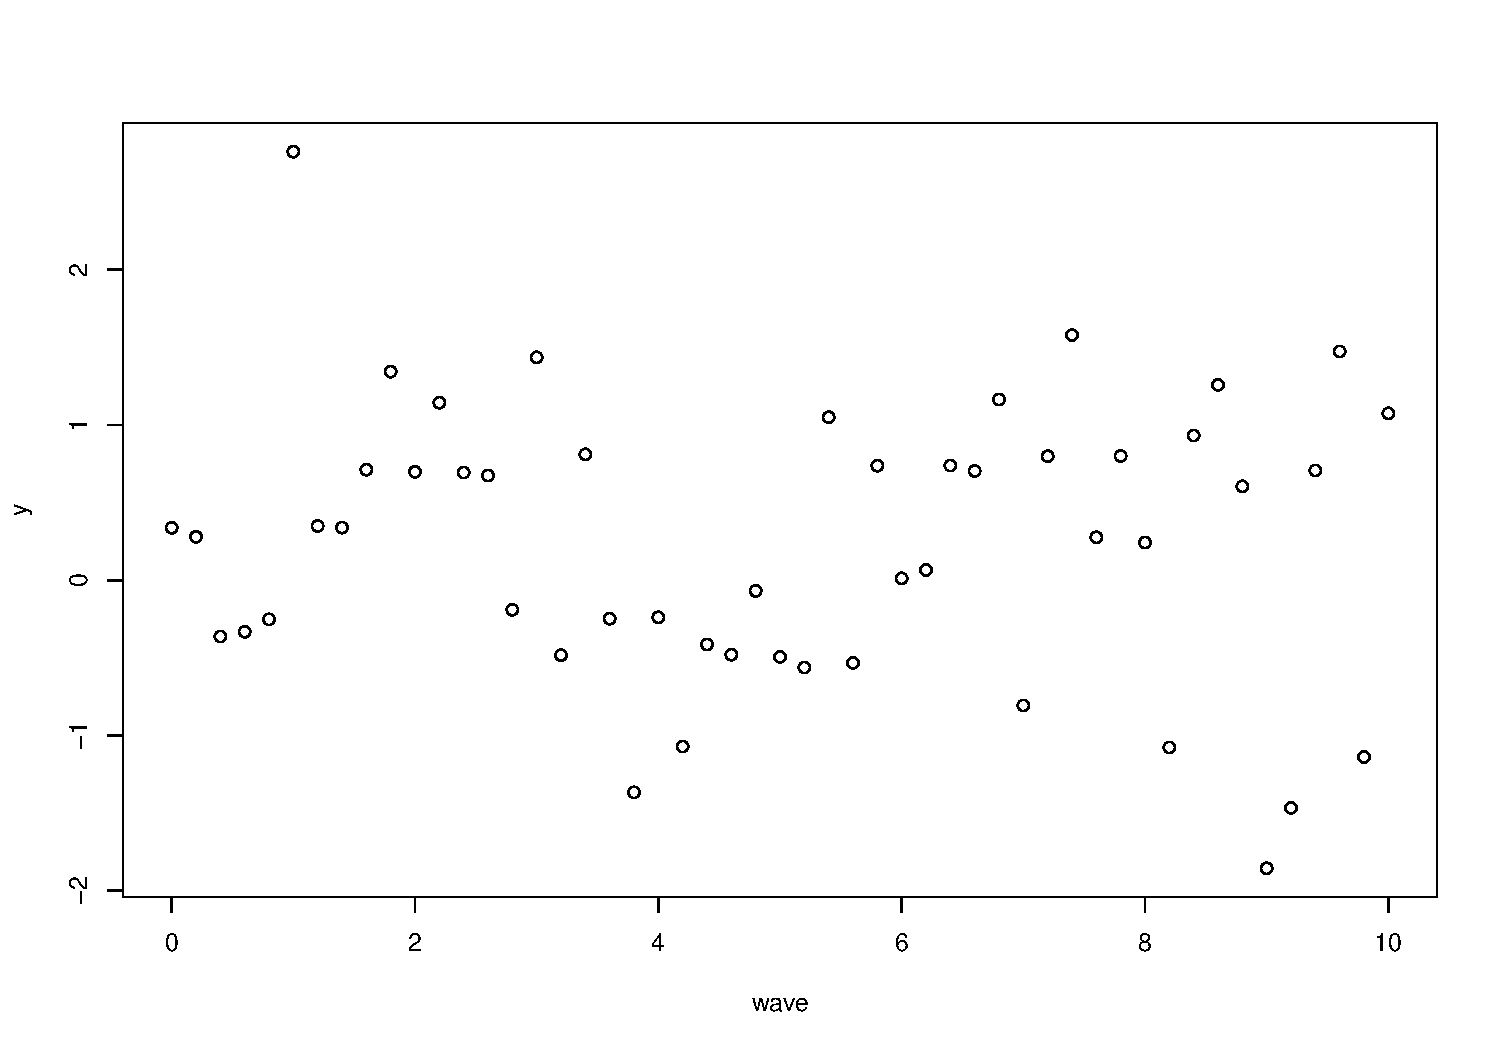
\includegraphics{CSwR22_Group2_BivariateSmoothing_Presentation_files/figure-beamer/unnamed-chunk-4-1.pdf}
\end{frame}

\begin{frame}{Implementation: Usage of the smoother}
\protect\hypertarget{implementation-usage-of-the-smoother}{}
\end{frame}

\begin{frame}{Implementation: Usage of the smoother (visualization)}
\protect\hypertarget{implementation-usage-of-the-smoother-visualization}{}
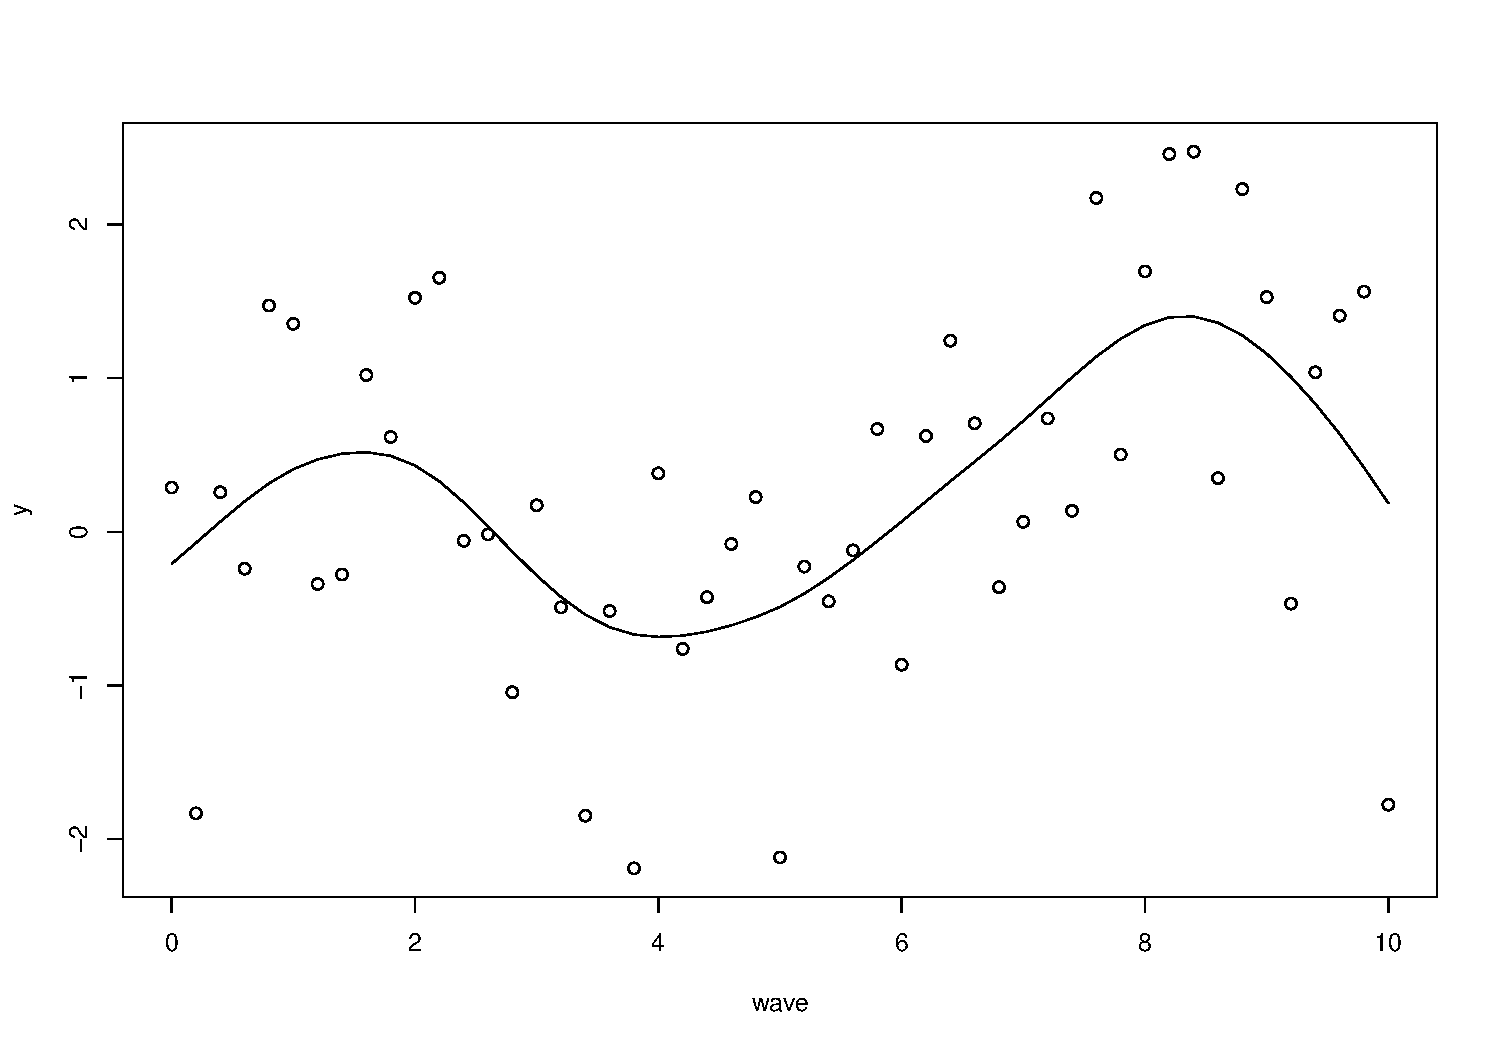
\includegraphics{CSwR22_Group2_BivariateSmoothing_Presentation_files/figure-beamer/unnamed-chunk-6-1.pdf}
\end{frame}

\begin{frame}{Error between the smoother and the original wave
(visualization)}
\protect\hypertarget{error-between-the-smoother-and-the-original-wave-visualization}{}
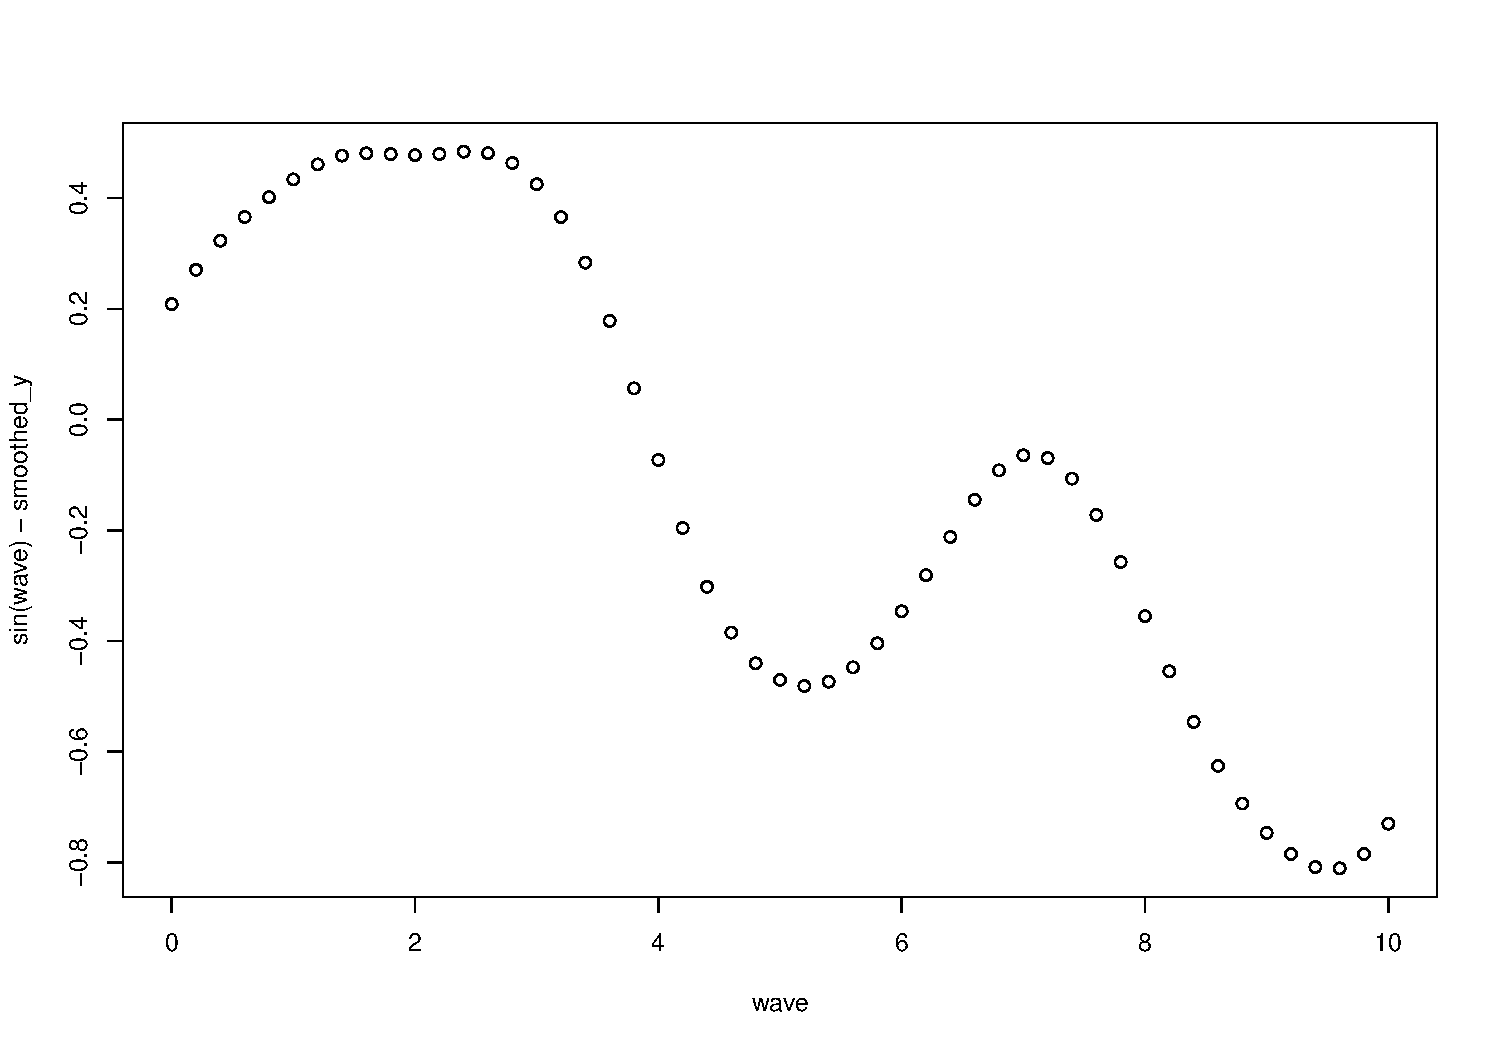
\includegraphics{CSwR22_Group2_BivariateSmoothing_Presentation_files/figure-beamer/unnamed-chunk-7-1.pdf}
\end{frame}

\begin{frame}[fragile]{MSE(sin(wave) - smoothed\_y)}
\protect\hypertarget{msesinwave---smoothed_y}{}
\begin{verbatim}
[1] 0.1847061
\end{verbatim}
\end{frame}

\begin{frame}[fragile]{Smoother with \texttt{smooth.spline}}
\protect\hypertarget{smoother-with-smooth.spline}{}
\begin{verbatim}
[1] 0.1938099
\end{verbatim}
\end{frame}

\begin{frame}[fragile]{Comparison with our smoother}
\protect\hypertarget{comparison-with-our-smoother}{}
\begin{verbatim}
[1] 0.001081587
\end{verbatim}
\end{frame}

\begin{frame}[fragile]{Benchmarking}
\protect\hypertarget{benchmarking}{}
\begin{verbatim}
[1] "Hello world"
\end{verbatim}
\end{frame}



\end{document}
